\documentclass[UTF8]{ctexart}
\usepackage{subfigure}
\usepackage{caption}
\usepackage{amsmath,bm}
\usepackage{amssymb}
\usepackage{pifont}
\usepackage{geometry}
\usepackage{graphicx}
\usepackage{gensymb}
\usepackage{wrapfig}
\usepackage{titlesec}
\usepackage{float}
\usepackage{diagbox}
\usepackage{fancyhdr}
\usepackage{color}
\usepackage{bm}
\usepackage{siunitx}
\usepackage{ulem}
\usepackage{CJKulem}
\pagestyle{plain}
\geometry{a4paper,scale=0.8}
\CTEXsetup[format+={\raggedright}]{section} 
\title{固物2020期末第二版——答案}
\author{Deschain}
\titlespacing*{\section}
{0pt}{0pt}{0pt}
\titlespacing*{\subsection}
{0pt}{0pt}{0pt}
\titlespacing*{\paragraph}
{0pt}{0pt}{0pt}
\titlespacing*{\subparagraph}
{0pt}{0pt}{0pt}
\titleformat*{\section}{\normalsize}
\begin{document}
\maketitle
% \section*{1.}
% (1)堆积比最大的晶格结构有\uline{\color{white} 面心立方}和\uline{\color{white} 六角密排}。\\
% (2)晶胞的两种定义方法:\uline{\color{white} 原胞}和\uline{\color{white} 单胞}。\\
% (3)写出除C之外的两种金刚石结构的半导体材料:\uline{\color{white} 硅和锗}。\\
% (4)计算晶体离子结合库仑势能要用到\uline{\color{white} 马德隆常数},它只与\uline{\color{white} 晶格结构}有关。\\
% (5)无限大自由空间电子$E-k$关系为\uline{\color{white} 抛物线型},切线\uline{\color{white} 斜率的变化率}与$\frac{1}{m}$成正比。
% (6)一价正负离子交错排列,形成一维晶格,平衡间距为$a$,只计近邻原子的作用,$U(r)=-\frac{q^2}{r}+\frac{b}{r^n}$,则$b=$
% \uline{\color{white} $\frac{(n-1)q^2}{a^3}$},刚性系数$\beta=$\uline{\color{white} $\frac{(n-1)q^2}{a^3}$}。\\
% (7)yz厚度为0.1cm的n型材料,沿x轴方向通50mA电流,沿z轴方向加0.5T磁场,得到0.4mV的电场。材料的霍尔系数为\uline{\color{white} 
% $-1.6\times10^{-5}m^3/C$},载流子浓度为\uline{\color{white} $3.9\times10^{23}m^{-3}$}。\\
% (8)PN结形成是半导体中载流子\uline{\color{white} 扩散}与\uline{\color{white} 漂移}的动态平衡过程。内建电场在PN结\uline{\color{white}
%  界面}处最强。空间电荷区宽度与掺杂浓度成\uline{\color{white} 反比}。偏压电流主要与\uline{\color{white} 少子}浓度变化有关。\\
% (9)索末菲自由电子模型中,二维材料的面积为S,则k空间的点阵密度为\uline{\color{white} $\frac{S}{4\pi^2}$},能量标度自由电子能态密度为
% \uline{\color{white} $\frac{Sm}{\pi\hbar^2}$}。\\
% (10)金属与N型半导体形成欧姆接触的条件是$\phi_M$\uline{\color{white} <}$\phi_N$,热平衡状态下,电子会流向\uline{\color{white} 半导体}。\\
% (11)有效质量包含\uline{\color{white} 周期势场}作用。在能带顶,电子的有效质量为\uline{\color{white} 负}(正/负)。能带顶的电子从外场得到
% 的动量\uline{\color{white} 小于}(大于/小于)交给金属的动量。\\
% (12)与索末菲模型相比,布洛赫电子考虑了晶体中的\uline{\color{white} 周期势场}对电子运动的影响。设简约波矢为$\vec{k}$,则$\psi(\vec{r}+\vec{R_n})=$
% \uline{\color{white} $e^{i\vec{k}\cdot\vec{R_n}}$}$\psi(\vec{r})$。考虑一维情况,$\psi_k(x)=-icos(\frac{4\pi x}{a})$,$a$是晶格常数,
% 则简约波矢为\uline{\color{white} 0}。\\
% (13)异质PN结若想获得更高电子注入比,需要N区带隙宽度\uline{\color{white} 大于}P区。\\
% (14)一块金刚石晶体中有2N个C原子,其包含\uline{\color{white} 3}支光学支色散曲线,\uline{\color{white} 3}支声学支色散曲线,每支有\uline{\color
% {white} $N$}个色散模式。\\
% (15)长光学支格波B和长声学支格波A,B反映了\uline{\color{white} 原胞内原子间的相对振动},A反映了\uline{\color{white} 所有原子的整体运动}。
% A振动的频率比B\uline{\color{white} 低}(高/低),平均声子数比B\uline{\color{white} 多}(多/少)。\\
% (16)常温下1mol NaCl热容为\uline{\color{white} $N_ak_B$},低温时,NaCl的热容随温度的\uline{\color{white} 3}次方减小。\\
% (17)体心立方晶格,晶格常数为a,体积为V,倒格子是\uline{\color{white} 面心立方}晶格。第一布里渊区体积为\uline{\color{white} $\frac{16\pi^3}{a^3}$}
% ,k的取值总数为\uline{\color{white} $\frac{2V}{a^3}$}。如果每个原子提供一个价电子,则0K时费米球半径为\uline{\color{white} $\frac{(6\pi)^{\frac{1}{3}}}{a}$}
% ,费米能量\uline{\color{white} $\frac{\hbar^2}{2ma^2}(6\pi^2)^{\frac{2}{3}}$}。\\
% (18)固体磁性分成\uline{\color{white} 抗磁性}、\uline{\color{white} 顺磁性}、\uline{\color{white} 铁磁性}、\uline{\color{white} 反铁磁性}、
% \uline{\color{white} 亚铁磁性}。忽略核磁矩,则原子磁矩主要来源于电子的\uline{\color{white} 轨道磁矩}、电子的\uline{\color{white} 自旋磁矩}和
% \uline{\color{white} 感生磁矩}。\\
% \section*{2.NaCl立方晶系,摩尔质量$58.5g/mol$,室温下的密度为$2.165g\cdot cm^3$。}
% (1)写出NaCl的晶体结构,并求出晶格常数$a$。\\
% (2)在晶格衍射实验中,测得最小衍射角为12度,求实验用的射线的波长。\\
% (3)描述第一布里渊区的形状,并求出第一布里渊区的体积。\\
% \section*{3.一维材料的$V(x)$满足$V(0)=V_1,V(\frac{a}{4})=V_2,V(\frac{a}{8})=V_3,\int_{-\frac{a}{2}}^{\frac{a}{2}}V(x)dx=0$。$a$是晶格常数,
% $V(x)$是偶函数并且是周期函数,第四级及以上的带隙为0。}
% (1)使用近自由电子近似,求第一、二、三条带隙的宽度。\\
% (2)画出简约布里渊区的能带图。\\
% (3)定性分析电子沿x轴正向受力为F时在k空间的运动,并标注。\\
% \section*{4. 300K时,$N-Al_xGa_{1-x}As$在左侧,$GaAs$在中间,$P-Al_xGa_{1-x}As$在右侧。左侧是N型重掺杂,掺杂浓度$N_D=1.0\times10^{19}cm^{-3}$;
% 中间是本征半导体;右侧是P型重掺杂,掺杂浓度$N_A=5.0\times10^{19}cm^{-3}$。$x=0.3$时,$GaAs$和$N-Al_xGa_{1-x}As$的禁带宽度分别为1.42eV、1.8eV,
% 本征载流子浓度分别为$2.1\times10^6cm^{-3}$、$2.1\times10^3cm^{-3}$,导带差$\Delta E_C=0.66\Delta E_g$。}
% (1)求$N-Al_xGa_{1-x}As$和$P-Al_xGa_{1-x}As$的费米能级相对于本征费米能级的位置。\\
% (2)定量计算$\Delta E_C,\Delta E_V$及接触电势差,画出能带图。\\
% \section*{5.长度为L的一维双原子链,刚性系数$\beta_1, \beta_2$,晶格常数为$a$,质量为$m$,只考虑近邻原子的作用,采用简谐近似。求出:}
% (1)运动方程;\\
% (2)色散曲线的表达式;\\
% (3)画出色散曲线示意图,标注边界和中心频率;\\
% (4)计算声学波波速的表达式和布里渊区中心的声学支格波的态密度。\\





答案:
\section*{1.填空题}
(1)\ding{172}面心立方\ding{173}六角密排\\
(2)\ding{172}原胞\ding{173}惯用晶胞\\
(3)\ding{172}硅\ding{173}锗\ding{174}共价键\\
(4)\ding{172}马德隆常数\ding{173}晶体结构\\
(5)\ding{172}抛物线型\ding{173}斜率的变化率\\
(6)\ding{172}$\frac{(n-1)q^2}{a^3}$\ding{173}$\frac{(n-1)q^2}{a^3}$\\
(7)\ding{172}$1.6\times10^{-5}$\ding{173}$3.90625\times10^{23}$\\
(8)\ding{172}扩散\ding{173}漂移\ding{174}反比\ding{175}少子\\
(9)\ding{172}$\frac{S}{4\pi^2}$\ding{173}$\frac{Sm}{\pi\hbar^2}$\\
(10)\ding{172}大于\ding{173}半导体\\
(11)\ding{172}周期势场\ding{173}负\ding{174}小于\\
(12)\ding{172}周期势场\ding{173}$e^{i\vec{k}\cdot\vec{R_n}}$\ding{174}0\\
(13)\ding{172}大于\\
(14)\ding{172}3\ding{173}3\ding{174}n\\
(15)\ding{172}原胞内原子间的相对振动\ding{173}所有原子的整体运动\\
(16)\ding{172}$N_ak_B$\ding{173}3\\
(17)\ding{172}面心立方\ding{173}$\frac{16\pi^3}{a^3}$\ding{174}$\frac{2V}{a^3}$\ding{175}$(\frac{6\pi^2}{a^3})^{\frac{1}{3}}$\ding{176}$\frac{\hbar^2}{2ma^2}(6\pi^2)^{\frac{2}{3}}$\\
(18)\ding{172}亚铁磁性\ding{173}反铁磁性\ding{174}感生磁矩\\
\section*{2.}
(1)面心立方
\begin{equation*}
    \begin{aligned}
        & a=\sqrt[3]{\frac{M}{\rho N_A}}=\sqrt[3]{\frac{58.5\times4}{2.165\times10^6\times6.02\times10^{23}}}=5.64\mathring{A}\\
    \end{aligned}
\end{equation*}
(2)
\begin{equation*}
    \begin{aligned}
        & \theta = 6\degree, d = \frac{a}{\sqrt3}, \lambda = 2dsin\theta = 0.681\mathring{A}\\
    \end{aligned}
\end{equation*}
(3)\\
立方体切去六角(切点为每条棱的中点)形成的十四面体。
\begin{equation*}
    \begin{aligned}
        & V = \frac{32\pi^3}{a^3} = 5.53\times10^{30}m^{-3}\\
    \end{aligned}
\end{equation*}
\section*{3.}
(1)
\begin{equation*}
    \begin{aligned}
        & V(x)=Acos(\frac{2\pi x}{a})+Bcos(\frac{4\pi x}{a})+Ccos(\frac{6\pi x}{a})\\
        & \begin{cases}
            A+B+C=V_1\\
            -B=V_2\\
            \frac{1}{\sqrt2}(A-C)=V_3\\
        \end{cases}\\
        & \begin{cases}
            A=\frac{1}{2}(V_1+V_2+\sqrt2 V_3)\\
            B=-V_2\\
            C=\frac{1}{2}(V_1+V_2-\sqrt2 V_3)\\
        \end{cases}\\
        & E_{g_1}=\lvert A\rvert = \frac{1}{2}(V_1+V_2+\sqrt2 V_3), E_{g_2}=\lvert B\rvert = V_2, E_{g_3}=\lvert C\rvert = 
        \frac{1}{2}(V_1+V_2-\sqrt2 V_3)\\
    \end{aligned}
\end{equation*}
(2,3)
\begin{wrapfigure}{l}{6cm}
    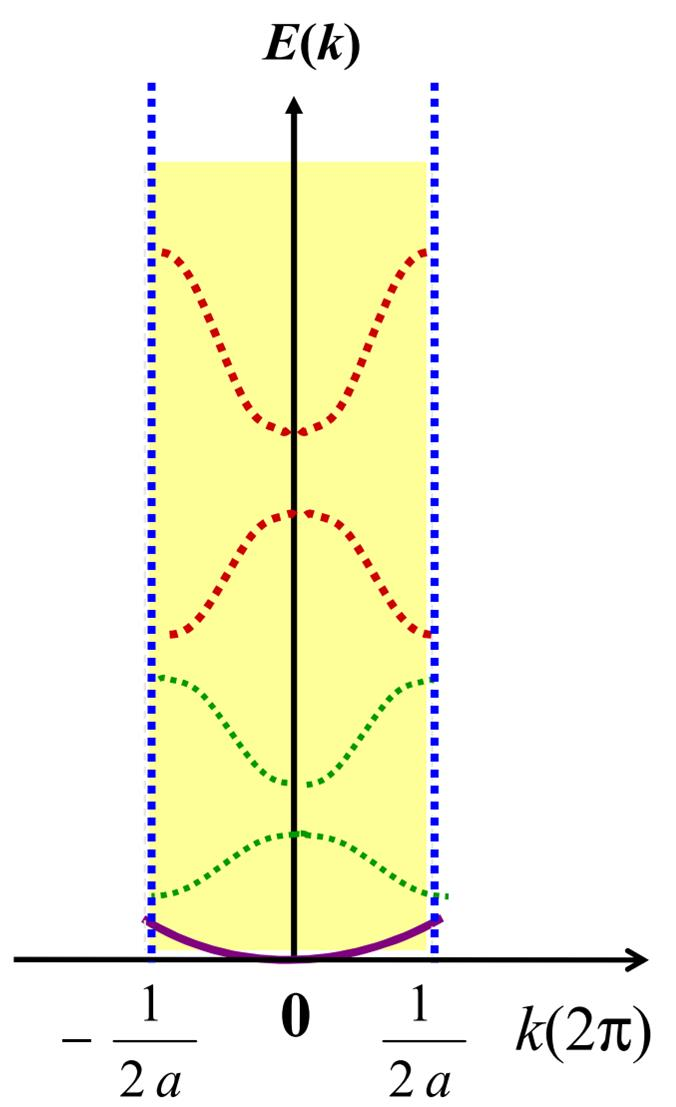
\includegraphics[width=3cm]{ans-3-2.jpg}
    \caption*{}
\end{wrapfigure}
在图中的某一条能带上,作k空间(k正向)的运动,并且是循环运动,从$-\frac{\pi}{a}$移出,从$\frac{\pi}{a}$移入。反向加速->反向减速->正向加速->正向减速。\\
\newline\newline\newline\newline\newline\newline\newline\newline\newline
\section*{4.}
(1)
\begin{equation*}
    \begin{aligned}
        & E_{Fn}=E_{Fi_2}+k_BTln(\frac{N_D}{n_{i2}})=E_{Fi_2}+0.935eV\\
        & E_{Fp}=E_{Fi_2}-k_BTln(\frac{N_A}{n_{i2}})=E_{Fi_2}-0.976eV\\ 
    \end{aligned}
\end{equation*}
(2)
\begin{figure}[H]
    \centering
    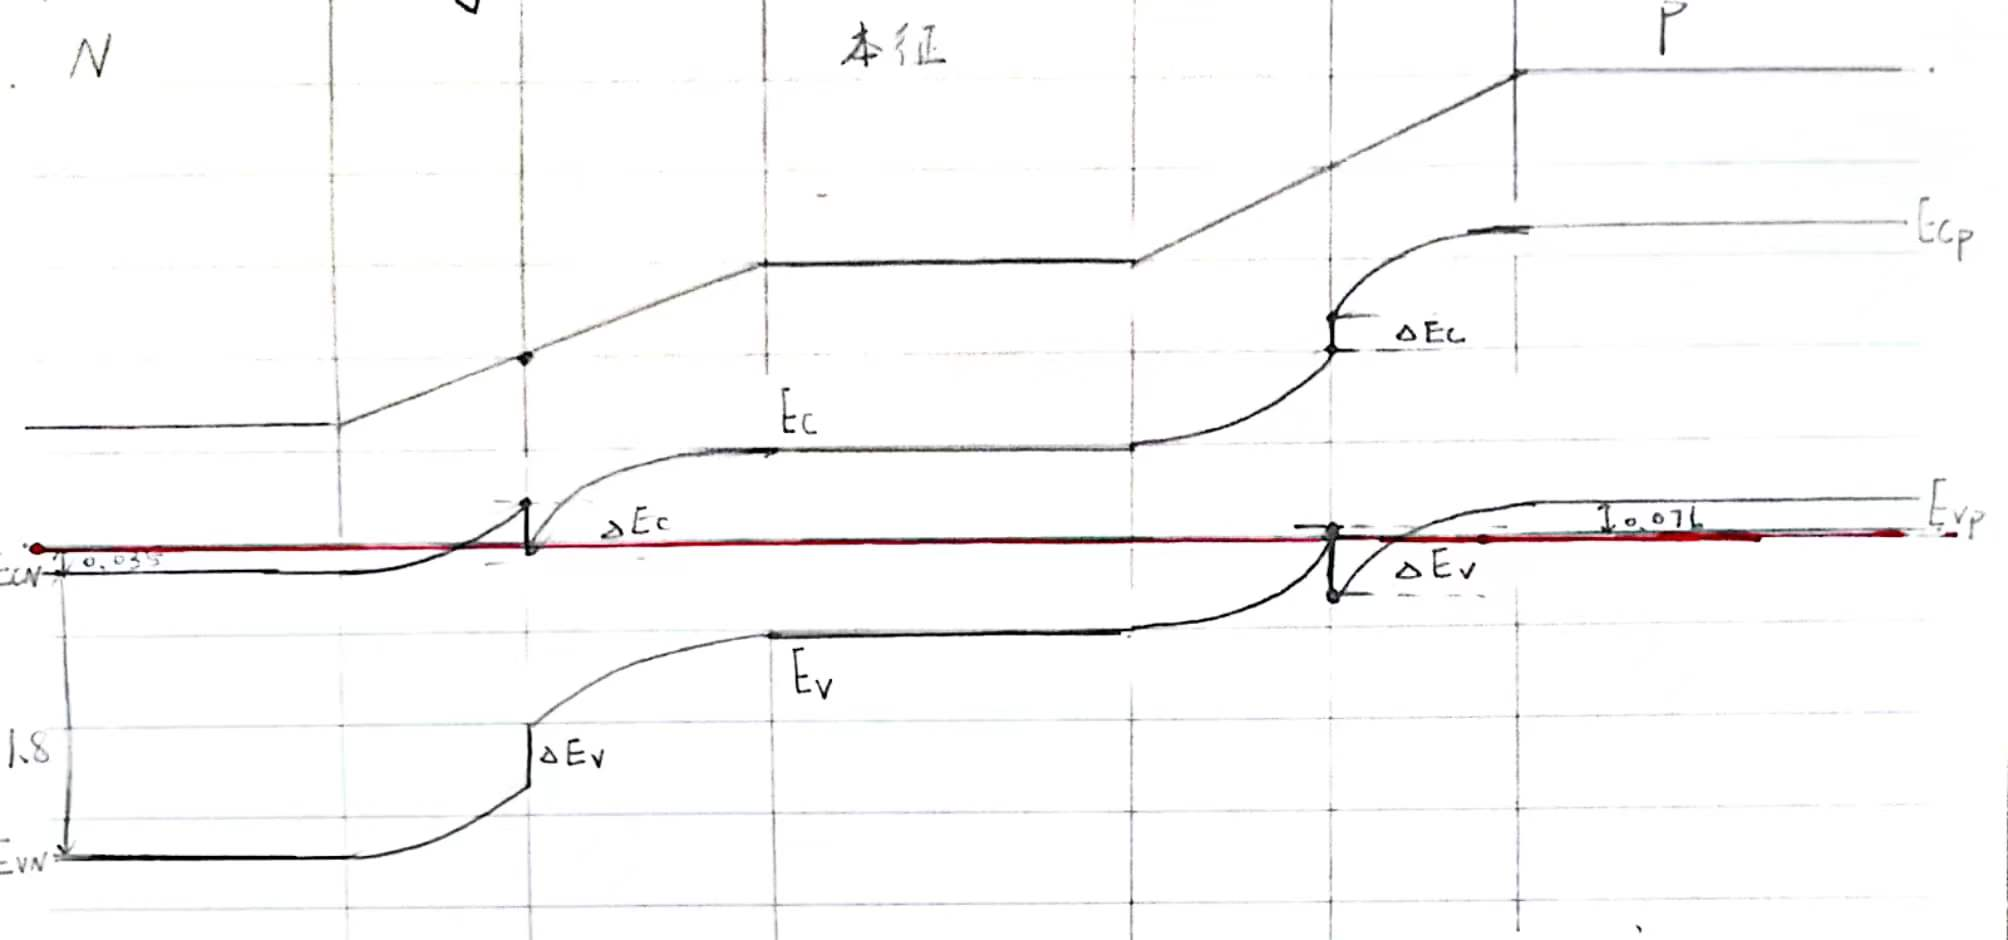
\includegraphics[width=8cm,height=4cm]{ans-4-2.jpg}
    \caption*{}
\end{figure}
\begin{equation*}
    \begin{aligned}
        & \Delta E_C=0.66\Delta E_g=0.66\times(1.80-1.42)=0.251eV\\
        & \Delta E_V=E_{g1}-E_{g2}-\Delta E_C=0.34\times(1.80-1.42)=0.129eV\\
        & V_{Dn} = E_{Fn} - E_{Fi1} = 0.996eV, V_{Dp} = E_{Fi1} - E_{F_p} = 0.915eV\\
    \end{aligned}
\end{equation*}
\section*{5.}
(1)
\begin{equation*}
    \begin{aligned}
        & m\ddot\mu_{2n}=-\beta_1(\mu_{2n}-\mu_{2n-1})-\beta_1(\mu_{2n}-\mu_{2n+1})\\
        & m\ddot\mu_{2n+1}=-\beta_2(\mu_{2n+1}-\mu_{2n})-\beta_1(\mu_{2n+1}-\mu_{2n+2})\\
    \end{aligned}
\end{equation*}
(2)
\begin{equation*}
    \begin{aligned}
        & \mu_{2n} = Ae^{i(\omega t-2nqa)}, \mu_{2n+1} = Be^{i(\omega t-(2n+1)qa)}\\
        & -m\omega^2A=-\beta_2(A-Be^{iaq})-\beta_1(A-Be^{-iaq})\\
        & -m\omega^2B=-\beta_1(B-Ae^{iaq})-\beta_2(B-Ae^{-iaq})\\
        & (m\omega^2 -\beta_1 -\beta_2)^2-[\beta_1^2+\beta_2^2+\beta_1\beta_2(e^{2iaq}+e^{-2iaq})]=0\\
        & \omega = \sqrt{\frac{1}{m}[\beta_1+\beta_2\pm\sqrt{\beta_1^2+\beta_2^2+2\beta_1\beta_2cos(2aq)}]}\\
    \end{aligned}
\end{equation*}
(3)
\begin{figure}[H]                                         
    \centering                                                
    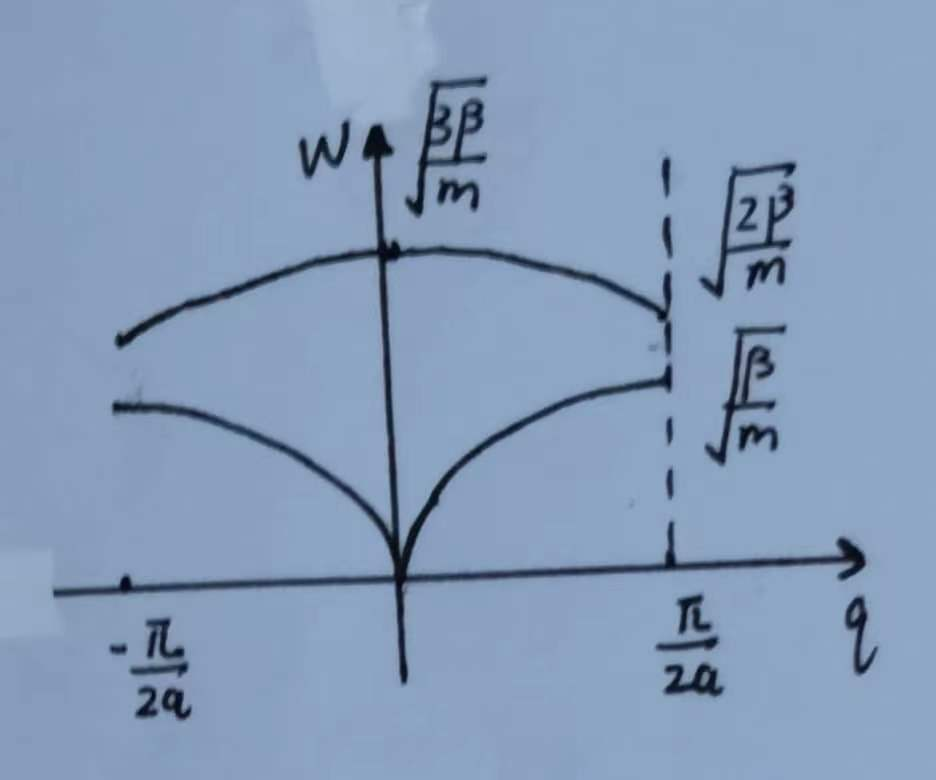
\includegraphics[width=5cm,height=4cm]{ans-5-3.jpg}       
    \caption*{}                                                                              
    \end{figure}
(4)
\begin{equation*}
    \begin{aligned}
        & v_a = \frac{d\omega}{dq}\lVert_{q=0}=a\sqrt{\frac{\beta_1\beta_2}{2m(\beta_1+\beta_2)}}\\
        & D(\omega) = \frac{L}{\pi v_a}=\frac{L}{\pi a}\sqrt{\frac{2m(\beta_1+\beta_2)}{\beta_1\beta_2}}\\
    \end{aligned}
\end{equation*}


\end{document}
